%-------------------------------------------------------------------------------
%% outhesis_template.tex
%% version 1.0
%% Chris McRaven <mcraven@physics.ou.edu>
%%
%% 'outhesis.cls' is a class file for a master or phd thesis that
%% conforms to the requirements of the graduate college at the
%% University of Oklahoma. This file is a hacked version of 'book.cls,'
%% that includes all of the formatting requirements set forth in
%% the document 'DissertationInstPacket.pdf' available at
%% http://gradweb.ou.edu/Current/Forms/doctoral/DissertationPagination.pdf
%%
%% This class file relies on a few packages to work.  You must have the
%% following packages installed:
%%  amsfonts, amsmath, amssymb, tikz, lineno, microtype, hyperref
%%
%% Most of these packages are included in distributions of latex.  If you
%% get a lot of errors when compiling, check that these packages are
%% installed.
%%
%% By default, the class file will conform to the requirements, but three
%% options are provided for assistance in proofing the document.
%%
%% linenumbers -- turns on linenumbers in the left margin
%% summarypage -- places a page at the beginning of the document listing 
%%                the number of tables, figures, and bibliography items.
%% hyperlinks -- hyperlinks the citations and references for easier
%%                navigation in the document in a reader which supports
%%                hyperlinks.
%%
%-------------------------------------------------------------------------------

\newcommand*{\ATLASLATEXPATH}{atlas_latex/}

%\documentclass[linenumbers,summarypage,hyperlinks]{outhesis}
%\documentclass[linenumbers,hyperlinks]{outhesis}
\documentclass[hyperlinks]{outhesis}
%\documentclass{outhesis}



%-------------------------------------------------------------------------------
% Extra packages:
%-------------------------------------------------------------------------------
% Style file with biblatex options for ATLAS documents.
\usepackage{\ATLASLATEXPATH atlasbiblatex}

% Useful macros
\usepackage{\ATLASLATEXPATH atlasphysics}
% See doc/atlas-physics.pdf for a list of the defined symbols.
% Default options are:
%   true:  journal, misc, particle, unit, xref
%   false: BSM, hion, math, process, other, texmf
% See the package for details on the options.


\usepackage[margin=1.0in]{geometry} % see geometry.pdf on how to lay out the page. There's lots.
%\usepackage{geometry} % see geometry.pdf on how to lay out the page. There's lots.
\usepackage{graphicx}
\usepackage{subcaption} %These packages gives the author the ability to have subfigures within figures, or subtables within table floats.
\usepackage{hyperref}
\usepackage{slashed} % Dirac slash notation
\usepackage{amsmath}
\usepackage{authblk}
\usepackage{multirow}

\geometry{a4paper} % or letter or a5paper or ... etc
% \geometry{landscape} % rotated page geometry

%\usepackage[english]{babel}
%\usepackage[utf8x]{inputenc}
%\usepackage{listings}
%\usepackage{graphicx}
%\usepackage{textpos}  % for putting logo
%\usepackage{color}    % for setting font color
%\usepackage{hyperref} % for url
%\usepackage{tikz}     % transparent background image
%\usepackage{eurosym}  % euro sign
%\usepackage{multirow} %
%\usepackage{appendixnumberbeamer} % count presentation slides only
%\usepackage{pbox} % new line in cell of table
%\usepackage{tabularx} % can change the table width

%\newcommand{\HRule}{\rule{\linewidth}{0.3mm}}

%%%%%
%%%%%
%\usepackage[explicit]{titlesec}
%\usepackage{fix-cm}
%\usepackage{lipsum}
%% numbered
%\titleformat{\chapter}
%  {\normalfont\LARGE\bfseries\filleft}
%  {}
%  {0em}
%  {%
%    \parbox[b]{\dimexpr\linewidth-2.5cm\relax}{#1}\hfill%
%    \parbox[b]{2cm}{\hfill{\fontsize{80}{96}\selectfont\thechapter}}%
%  }
%% unnumbered
%\titleformat{name=\chapter,numberless}
%  {\normalfont\LARGE\bfseries\filleft}
%  {}
%  {0em}
%  {\parbox[b]{\dimexpr\linewidth-2.5cm\relax}{#1}}
%% spacing
%\titlespacing*{\chapter}
%  {0pt}{50pt}{40pt}
%%%%%
%%%%%  


\usepackage[toc]{appendix}
\usepackage{xspace}
%\usepackage{subfigure}
%\usepackage{subcaption}
%\usepackage{slashed}
%\usepackage{graphicx}
\usepackage[labelsep=colon,labelfont=bf,font=singlespacing,width=\textwidth,compatibility=false]{caption}
\usepackage{booktabs}
\usepackage{multirow,bigdelim}
\usepackage[compat=1.1.0]{tikz-feynman}

% For a bibliography style, you must have the appropriate .bst file
% \bibliographystyle{apj}
%\bibliographystyle{prsty}
%\bibliographystyle{atlasBibStyleWithTitle}

%\usepackage{thesis-def}


%-------------------------------------------------------------------------------
% Content
%-------------------------------------------------------------------------------
 
%%% BEGIN DOCUMENT
\begin{document}

%% Place Dissertation information here
\author{Yu-Ting Shen}
\university{University of Oklahoma}
\college{Graduate College}
\department{Homer L. Dodge Department of Physics and Astronomy}
\title{This is the thesis title}
\address{Norman, Oklahoma}
\yr{2017}
\dgname{Doctor of Philosophy}
%% List your committee members here
\committee{{Dr. Patrick Skubic, Chair}, Dr. Michael Strauss, {Dr. Ron Kantowski}, Dr. Deborah Watson, {Dr. S. Lakshmivarahan}}

%% Put your dedication here. This is completely optional. Delete it if you don't need it.
\begin{dedication}
To my past, present, and future family.

\begin{quotation}
\raggedright{\emph{``You're braver than you believe, and stronger than you seem, and smarter than you think.''}} \\
\raggedleft{- A.A. Milne, Christopher Robin} 
\end{quotation}

\end{dedication}

%% Put your acknowledgements here. This is completely optional. Delete it if you don't need it.
\begin{acknowledgements}
I would like to deeply thank all of my teachers and professors over the 20 years of my academic journey, for instilling in me a deep, unquenchable desire to learn. 
\begin{quotation}
\raggedright{\emph{``If you don't know, the thing to do is not to get scared, but to learn.''}} \\
\raggedleft{- Ayn Rand, Atlas Shrugged}
\end{quotation}

I would also like to thank all of my family and friends who have helped motivate and encourage me in my pursuit of this degree. 
\begin{quotation}
\raggedright{\emph{``It's the job that's never started as takes longest to finish.''}} \\
\raggedleft{- J.R.R. Tolkien, The Lord of the Rings}
\end{quotation}

Lastly, I would like to thank my wife for not only supporting me through the entire process, but actually pushing me to be the best me I could be. Thank you for living this adventure with me!
\begin{quotation}
\raggedright{\emph{``I am a wife-made man.''}} \\
\raggedleft{- Danny Kaye} 
\end{quotation}
\begin{quotation}
\raggedright{\emph{``I knew when I met you an adventure was going to happen.''}} \\
\raggedleft{- A.A. Milne, Winnie the Pooh} 
\end{quotation}
\end{acknowledgements}

%% Put your abstract here.
\begin{abstract}
Here is the abstract
\end{abstract}

\frontmatter

\maketitle

\mainmatter

\hypersetup{linkcolor=blue}

%% You can put any part of the text in separate file with 
%% the \input{} command. This keeps the master document simpler.

\chapter{Introduction}
\label{chapter:introduction}
\graphicspath{{figures/introduction/}}
The Standard Model of particle physics (SM) describes various phenomena of particle physics.
The discovery of the Higgs boson ($H$) by the ATLAS and CMS collaboration at CERN completes the missing part of the SM prediction~\cite{Aad:2012tfa, Chatrchyan:2012xdj}.
However, there are several open challenges that cannot be explained by the SM, such as hierarchy problem~\cite{Weinberg:1975gm, Gildener:1976ai, Susskind:1978ms} and the dark matter candidate.
In order to answer those questions, a new theory extending the SM is necessary.
Supersymmetry (SUSY)~\cite{Wess:1973kz, Wess:1974tw, Golfand:1971iw, Martin:1997ns} is the most promising extensions of the SM.
SUSY, which is a spacetime symmetry, introduces the superpartners of SM particles (sparticles) with spin differing by one-half unit with respect to the SM partners.
The sparticles provide a potential solution to the hierarchy problem.
If $R$-parity is conserved~\cite{Fayet:1976et, Fayet:1977yc, Farrar:1978xj}, the sparticles are produced in pairs and the lightest SUSY particle (LSP) is stable providing a candidate for dark matter.

The charginos $\widetilde{\chi}^{\pm}_{1,2}$ and neutralinos $\widetilde{\chi}^{0}_{1,2,3,4}$ are the mass eigenstates in the order of increasing masses and collectively referred to as electroweakinos.
They are the mixture of the bino $\widetilde{B}$, winos $\widetilde{W}$, and Higgsinos $\widetilde{H}_{u,d}$ which are the superpartners of the $U(1)$, $SU(2)$ gauge bosons, and the Higgs bosons, respectively.
The charginos and neutralinos can decay into leptons and LSPs via $W$, $Z$, $H$ or sleptons $\widetilde{\ell}$.
In many SUSY models, the lightest neutralino $\widetilde{\chi}^{0}_{1}$ is the LSP.
The LSP would not be detected and results in significant missing transverse energy \MET.

The compressed scenarios refer to the small mass differences between heavier SUSY particles and the LSP.
For example, the mass differences between the heavier electroweakino states $\widetilde{\chi}^{0}_{2}$, $\widetilde{\chi}^{\pm}_{1}$ and the wino- or Higgsino-dominated LSP $\widetilde{\chi}^{0}_{1}$ range from a few {\MeV} to tens of {\GeV} depending on the composition of the mixture.
The $\widetilde{B}$, $\widetilde{W}$, and $\widetilde{H}$ composition of the $\widetilde{\chi}^{0}_{1}$ have an influence on the degree of compression.
Figure~\ref{fig:intro_LSP_composition} shows the composition of the lightest neutralino in a MSSM scan of the electroweakino sector~\cite{Aaboud:2016wna}.
Based on naturalness arguments~\cite{Barbieri:1987fn, deCarlos:1993rbr}, the Higgsino mass parameter $\mu$, the bino and wino mass parameters $M_{1}$ and $M_{2}$ satisfy $|\mu| \ll |M_{1}|, |M_{2}|$ leading to the three electroweakinos $\widetilde{\chi}^{0}_{1}$, $\widetilde{\chi}^{\pm}_{1}$, and $\widetilde{\chi}^{0}_{2}$ being dominated by the Higgsino.

\begin{figure}[htbp]
    \begin{center}
        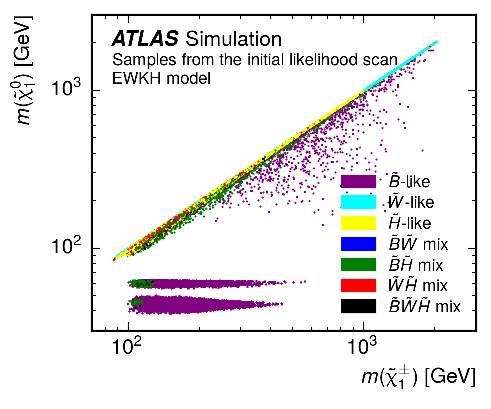
\includegraphics[scale=1.0]{LSP_composition.pdf}
        \caption{The scatter plot in the $m(\widetilde{\chi}^{0}_{1})$ vs $m(\widetilde{\chi}^{\pm}_{1})$ plane~\cite{Aaboud:2016wna}.
        The color encodes the $\widetilde{\chi}^{0}_{1}$ composition.
        The Higgsino-dominated LSPs are colored in yellow and along the $\widetilde{\chi}^{0}_{1}$-$\widetilde{\chi}^{\pm}_{1}$ diagonal.}
        \label{fig:intro_LSP_composition}
    \end{center}
\end{figure}

This dissertation focuses on searching for electroweak production of SUSY particles in compressed scenarios with exactly two low-momentum same-flavor opposite-charged leptons (electron and muon) in final states and missing transverse momentum $\textbf{p}_{\text{T}}^{\text{miss}}$.
This search uses proton-proton collision data at $\sqrt{s} = 13$~{\TeV} recorded by the ATLAS detector at the Large Hadron Collider (LHC)~\cite{Evans:2008zzb} in 2015 and 2016, corresponding to a total integrated luminosity of 36.1~\ifb.
Figure~\ref{fig:intro_feynman_diagrams} shows the Feynman diagrams representing the electroweakino productions with two leptons final state in association with an initial state radiated jet.
Same-flavor opposite-charged leptons come from the $\widetilde{\chi}^{0}_{2}$ decays in the $\widetilde{\chi}^{0}_{2} \widetilde{\chi}^{\pm}_{1}$ and $\widetilde{\chi}^{0}_{2} \widetilde{\chi}^{0}_{1}$ productions, and from the $\widetilde{\chi}^{\pm}_{1}$ decays in the $\widetilde{\chi}^{\pm}_{1} \widetilde{\chi}^{\mp}_{1}$ production.
The two leptons can be reconstructed in the detector and carry small transverse momentum  \pt.
However, the two LSPs are invisible and back-to-back in the rest frame of their parent electroweakinos.
Because they carry large momentum, the missing transverse energy \met is relatively large.
Similar searches have been performed using $\sqrt{s} = 8$~{\TeV} and $\sqrt{s} = 13$~{\TeV} by the ATLAS~\cite{Aad:2014vma, Aad:2014nua, Aad:2015eda, Aaboud:2016wna} and CMS~\cite{Khachatryan:2014qwa, Khachatryan:2015pot, Sirunyan:2017lae} experiments.
Combining with the results from the LEP experiments, the mass limits for sleptons and charginos are $m(\widetilde{e}_{R}) > 73$~{\GeV}, $m(\widetilde{\mu}_{R}) > 94.6$~{\GeV}, and $m(\widetilde{\chi}^{\pm}_{1}) > 103.5$~{\GeV} or 92.4~{\GeV} depending on the $\Delta m(\widetilde{\chi}^{0}_{1}, \widetilde{\chi}^{\pm}_{1})$.

\begin{figure}[htbp]
    \begin{center}
        \begin{subfigure}[b]{0.32\textwidth}
            \begin{center}
                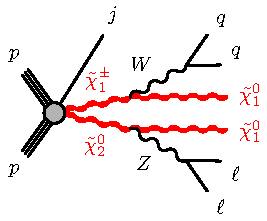
\includegraphics[scale=1.0]{C1N2-llqqN1N1g-WZ.pdf}
                \caption{The $\widetilde{\chi}^{0}_{2} \widetilde{\chi}^{\pm}_{1}$ production.}
            \end{center}
        \end{subfigure}%
        \begin{subfigure}[b]{0.32\textwidth}
            \begin{center}
                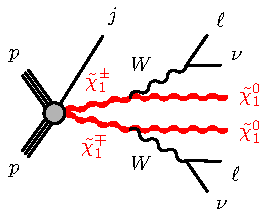
\includegraphics[scale=1.0]{C1C1-llvvN1N1g-WW.pdf}
                \caption{The $\widetilde{\chi}^{\pm}_{1} \widetilde{\chi}^{\mp}_{1}$ production.}
            \end{center}
        \end{subfigure}
        \begin{subfigure}[b]{0.32\textwidth}
            \begin{center}
                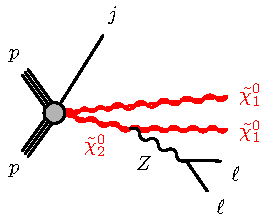
\includegraphics[scale=1.0]{N2N1-jllN1N1-Z.pdf}
                \caption{The $\widetilde{\chi}^{0}_{2} \widetilde{\chi}^{0}_{1}$ production.}
            \end{center}
        \end{subfigure}
    \end{center}
    \caption{The Feynman diagrams representing the two leptons final state of (a) $\widetilde{\chi}^{0}_{2} \widetilde{\chi}^{\pm}_{1}$, (b) $\widetilde{\chi}^{\pm}_{1} \widetilde{\chi}^{\mp}_{1}$, (c) $\widetilde{\chi}^{0}_{2} \widetilde{\chi}^{0}_{1}$ productions.}
    \label{fig:intro_feynman_diagrams}
\end{figure}

This dissertation has the following structure.
An introduction is given in Chapter~\ref{chapter:introduction} followed by theoretical foundations in Chapter~\ref{chapter:standard_model} and \ref{chapter:Supersymmetry}.
The experiment facilities are described in Chapter~\ref{chapter:altas_experiment}.
The data and Monte Carlo samples used are detailed in Chapter~\ref{chapter:data}.
Chapter~\ref{chapter:event_reconstruction_and_selection} presents the event reconstruction and the signal region selection.
The background estimation and the systematic uncertainties are discussed in Chapter~\ref{chapter:bkg_estimation}.
The results and interpretation are reported in Chapter~\ref{chapter:results}.
Finally, the conclusions are summarized in Chapter~\ref{chapter:conclusion}.



\chapter{The Standard Model}
\label{chapter:the_standard_model}
\graphicspath{{figures/the_standard_model/}}
This chapter outlines the theoretical and mathematical concepts of modern particle physics.
The Standard Model (SM) is the well-tested and most successful theory to describe the nature of the elementary particles and their interactions.
An overview of the SM is given in the Section \ref{sec: sm}.
More detail about the SM can be found in various 


The theories and discoveries of thousands of physicists since the 1930s have resulted in a remarkable insight into the fundamental structure of matter: everything in the universe is found to be made from a few basic building blocks called fundamental particles, governed by four fundamental forces. Our best understanding of how these particles and three of the forces are related to each other is encapsulated in the Standard Model of particle physics. Developed in the early 1970s, it has successfully explained almost all experimental results and precisely predicted a wide variety of phenomena. Over time and through many experiments, the Standard Model has become established as a well-tested physics theory.


\section{The Standard Model of Particle Physics} \label{sec: sm}
Developed in the early 1970s, the Standard Model of particle physics has successfully explained almost all experimental results and precisely predicted a wide variety of phenomena.
It is currently the most accurate description of elementary particles and their interactions.
It presents a combination of quantum mechanics and relativity theory to form a relativistic quantum field theory of the particles and the forces of our nature.






Matter particles

All matter around us is made of elementary particles, the building blocks of matter. These particles occur in two basic types called quarks and leptons. Each group consists of six particles, which are related in pairs, or “generations”. The lightest and most stable particles make up the first generation, whereas the heavier and less stable particles belong to the second and third generations. All stable matter in the universe is made from particles that belong to the first generation; any heavier particles quickly decay to the next most stable level. The six quarks are paired in the three generations – the “up quark” and the “down quark” form the first generation, followed by the “charm quark” and “strange quark”, then the “top quark” and “bottom (or beauty) quark”. Quarks also come in three different “colours” and only mix in such ways as to form colourless objects. The six leptons are similarly arranged in three generations – the “electron” and the “electron neutrino”, the “muon” and the “muon neutrino”, and the “tau” and the “tau neutrino”. The electron, the muon and the tau all have an electric charge and a sizeable mass, whereas the neutrinos are electrically neutral and have very little mass.
Forces and carrier particles

There are four fundamental forces at work in the universe: the strong force, the weak force, the electromagnetic force, and the gravitational force. They work over different ranges and have different strengths. Gravity is the weakest but it has an infinite range. The electromagnetic force also has infinite range but it is many times stronger than gravity. The weak and strong forces are effective only over a very short range and dominate only at the level of subatomic particles. Despite its name, the weak force is much stronger than gravity but it is indeed the weakest of the other three. The strong force, as the name suggests, is the strongest of all four fundamental interactions.
Three of the fundamental forces result from the exchange of force-carrier particles, which belong to a broader group called “bosons”. Particles of matter transfer discrete amounts of energy by exchanging bosons with each other. Each fundamental force has its own corresponding boson – the strong force is carried by the “gluon”, the electromagnetic force is carried by the “photon”, and the “W and Z bosons” are responsible for the weak force. Although not yet found, the “graviton” should be the corresponding force-carrying particle of gravity. The Standard Model includes the electromagnetic, strong and weak forces and all their carrier particles, and explains well how these forces act on all of the matter particles. However, the most familiar force in our everyday lives, gravity, is not part of the Standard Model, as fitting gravity comfortably into this framework has proved to be a difficult challenge. The quantum theory used to describe the micro world, and the general theory of relativity used to describe the macro world, are difficult to fit into a single framework. No one has managed to make the two mathematically compatible in the context of the Standard Model. But luckily for particle physics, when it comes to the minuscule scale of particles, the effect of gravity is so weak as to be negligible. Only when matter is in bulk, at the scale of the human body or of the planets for example, does the effect of gravity dominate. So the Standard Model still works well despite its reluctant exclusion of one of the fundamental forces.
So far so good, but...

...it is not time for physicists to call it a day just yet. Even though the Standard Model is currently the best description there is of the subatomic world, it does not explain the complete picture. The theory incorporates only three out of the four fundamental forces, omitting gravity. There are also important questions that it does not answer, such as “What is dark matter?”, or “What happened to the antimatter after the big bang?”, “Why are there three generations of quarks and leptons with such a different mass scale?” and more. Last but not least is a particle called the Higgs boson, an essential component of the Standard Model.
On 4 July 2012, the ATLAS and CMS experiments at CERN's Large Hadron Collider (LHC) announced they had each observed a new particle in the mass region around 126 GeV. This particle is consistent with the Higgs boson but it will take further work to determine whether or not it is the Higgs boson predicted by the Standard Model. The Higgs boson, as proposed within the Standard Model, is the simplest manifestation of the Brout-Englert-Higgs mechanism. Other types of Higgs bosons are predicted by other theories that go beyond the Standard Model.
On 8 October 2013 the Nobel prize in physics was awarded jointly to François Englert and Peter Higgs "for the theoretical discovery of a mechanism that contributes to our understanding of the origin of mass of subatomic particles, and which recently was confirmed through the discovery of the predicted fundamental particle, by the ATLAS and CMS experiments at CERN's Large Hadron Collider."
So although the Standard Model accurately describes the phenomena within its domain, it is still incomplete. Perhaps it is only a part of a bigger picture that includes new physics hidden deep in the subatomic world or in the dark recesses of the universe. New information from experiments at the LHC will help us to find more of these missing pieces.


\chapter{Suppersymmetry}
\label{chapter:Suppersymmetry}
\graphicspath{{figures/Suppersymmetry/}}
\input{chapter_Suppersymmetry}


\chapter{The ATLAS Experiment at LHC}
\label{chapter:altas_experiment}
\graphicspath{{figures/atlas_experiment/}}
The European Organization for Nuclear Research (CERN\footnote{The name CERN is derived from the acronym for the French Conseil Europ\'{e}en pour la Recherch Nucl\'{e}aire}) was founded in 1954 and is based in the suburb of Geneva on the Franco\textendash Swiss border.
The main function of CERN is to provide particle accelerators and detectors for high-energy physics research.
The physicists and engineers at CERN are probing the fundamental structure of the universe using the world's largest and most complex scientific facility \textemdash \ the Large Hadron Collider (LHC)~\cite{1748-0221-3-08-S08001}.
In the LHC, the particles are boosted to high energies and collide at close to the speed of light.
The results of the collisions are recorded by the various detectors.
There are seven experiments at the LHC.
The biggest of these experiments are ATLAS (A Toroidal LHC ApparatuS)~\cite{1748-0221-3-08-S08003} and CMS (Compact Muon Solenoid)~\cite{1748-0221-3-08-S08004} which use general-purpose detectors to investigate a broad physics programme ranging from the search for the Higgs boson to extra dimensions and particles that could make up dark matter.
The ALICE (A Large Ion Collider Experiment)~\cite{1748-0221-3-08-S08002} experiment is designed to study the physics of quark-gluon plasma form and the LHCb (Large Hadron Collider beauty)~\cite{1748-0221-3-08-S08005} experiment specializes in investigating of CP violation by studying the $b$-quark.
These four detectors sit underground in huge caverns of the LHC ring.
The rest three experiments, TOTEM~\cite{1748-0221-3-08-S08007}, LHCf~\cite{1748-0221-3-08-S08006}, and MoEDAL~\cite{Pinfold:1181486}, are smaller.
The TOTEM (TOTal Elastic and diffractive cross section Measurement)~\cite{1748-0221-3-08-S08007} experiment aims at the measurement of total cross section, elastic scattering, and diffractive dissociation.
The LHCf (Large Hadron Collider forward)~\cite{1748-0221-3-08-S08006} experiment is intended to measure the neutral particle produced by the collider using the forward particles.
The prime motivation of the MoEDAL (Monopole and Exotics Detector at the LHC)~\cite{Pinfold:1181486} experiment is to search directly for the magnetic monopole.

\section{The Large Hadron Collide}

The LHC~\cite{1748-0221-3-08-S08001} is the world's largest and most powerful accelerator which accelerates and collides protons in a 26.7~km circumference crossing the Franco\textendash Swiss border 100 m underground.
Built in the tunnel of the former LEP (Large Electron\textendash Positron), the LHC is capable of colliding protons as well as heavy ions.
Comparing with the LEP which collides electrons and positrons, the advantage of the LHC is the lower energy loss \footnote{The energy loss for protons is about eleven orders of magnitude smaller than the electrons} in the synchrotron radiation, such that higher energies can be reached by the LHC.
The LHC is designed for collisions at a centre-of-mass energy $\sqrt{s}=14$~{\TeV} and an instantaneous luminosity of $\mathcal{L} =10^{34}~\textrm{cm}^{-2}\textrm{s}^{-1}$.
Figure~\ref{fig:CERN_accelerator_complex} shows the infrastructure of the LHC and the pre-accelerator system.

\begin{figure}[htbp]
\begin{center}
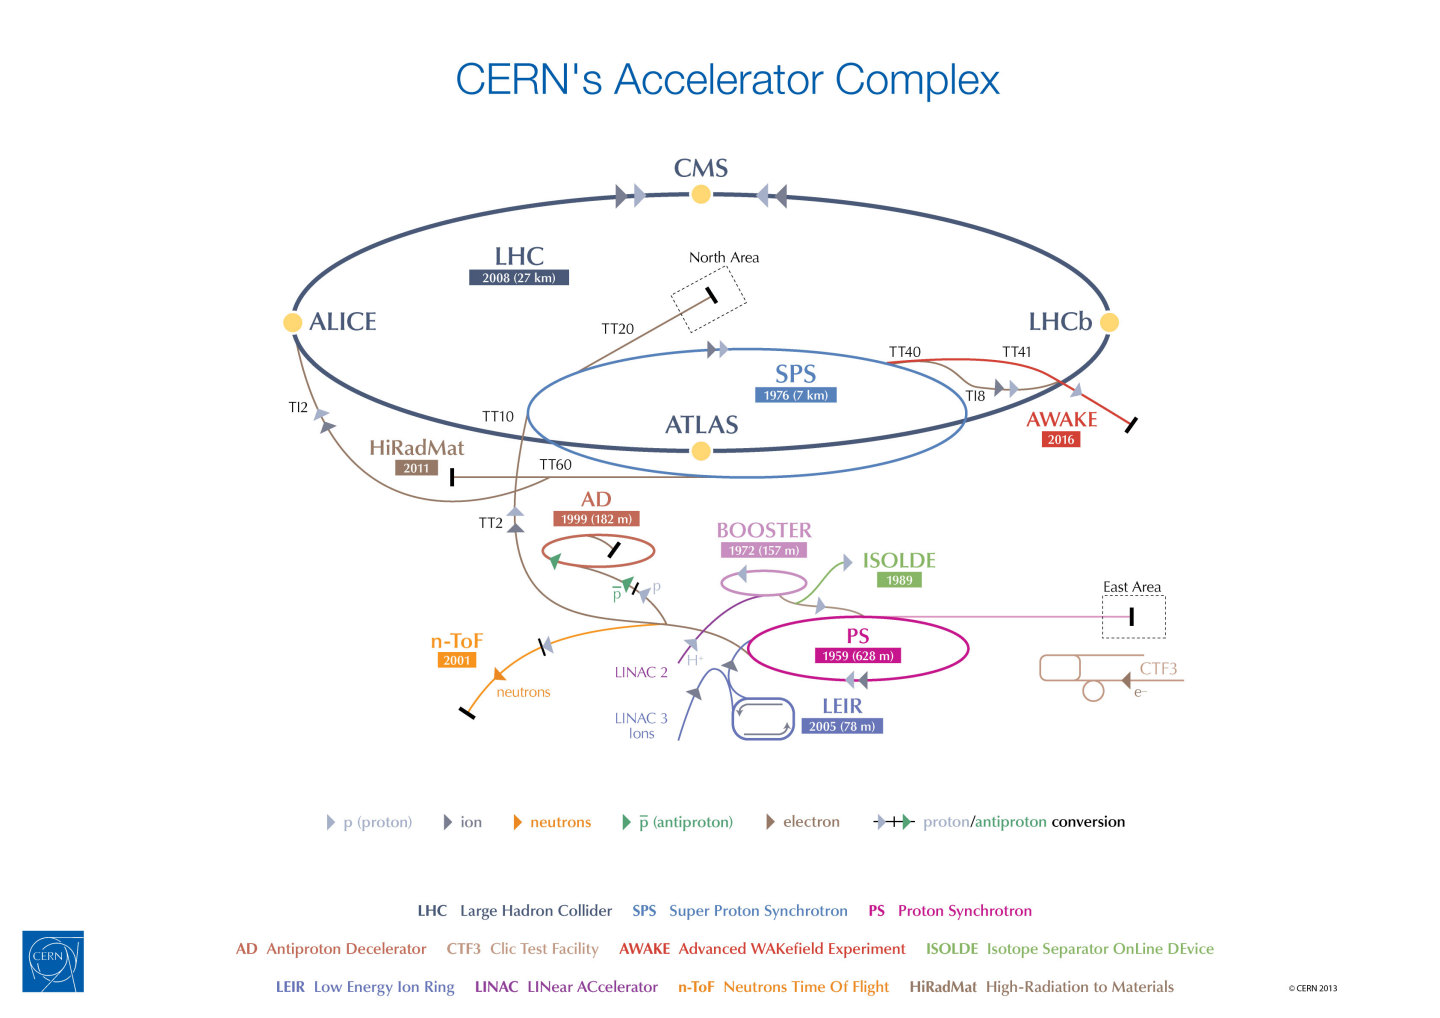
\includegraphics[scale=0.4]{CERN's-accelerator-complex2013.jpg}
\caption{The accelerator complex at CERN~\cite{Marcastel:1621583}.}
\label{fig:CERN_accelerator_complex}
\end{center}
\end{figure}

The protons are extracted by ionization from a hydrogen source and are accelerated to 50~{\MeV} by the linear accelerator LINAC2.
Then they are injected into the Proton Synchrotron Booster (PSB) where the proton energies are increased to 1.4~{\GeV} before they enter the Proton Synchrotron (PS) which accelerates the protons to 25~{\GeV}.
Next, the proton energies are increasing to 450~{\GeV} in the Super Proton Synchrotron (SPS). 
Finally, the protons are split into two beams and enter the LHC where the two beams run in two adjacent beam pipes with opposite directions.
In order to keep the protons on the circular trajectory in the LHC, 1232 superconducting dipole magnets~\cite{1288863} generate a magnetic field strength of 8.33~T to bend the proton beams in eight arcs.
Additionally, 392 quadrupole magnets~\cite{1288863} are installed to focus the beam.
A cryogenic system running with super-fluid helium-4 is used to cool down the superconducting magnets to a temperature of 1.7~K.

For a given physics process, the event rate is proportional to the cross section $\sigma$ of this process.
\begin{equation}
\frac{dN}{dt} = \mathcal{L}\cdot\sigma
\end{equation}
where $N$ is the number of events and $\mathcal{L}$ denotes the luminosity of the beam.
The luminosity of the beam, $\mathcal{L}$ can be calculated by
\begin{equation}
\mathcal{L} = \frac{N^{2} f}{4 \pi \sigma_{x} \sigma_{y}} \cdot F
\end{equation}
where $N$ is the number of protons, $f$ is the bunches crossing frequency, and the $\sigma_{x}$ and $\sigma_{y}$ are the $x$ and $y$ components for cross section $\sigma$.
The geometric luminosity reduction factor, $F$, is related to the crossing angle at the Interaction Point (IP).
Considering a beam consisting of $1.15 \times 10^{11}$ protons with bunching spacing of 25~ns, the transversal size of the bunch at Interaction Pointe $16\times 10^{-4}$~cm, and taking the geometric luminosity reduction factor as 1, the design luminosity of $10^{34}$~cm$^{-2}$s$^{-1}$ can be reached.

The first beam was circulated through the collider on the morning of 10 September 2008~\cite{CERN-COURIER-Sep192008}.
However, a magnet quench incident occurred on 19 September 2008 and caused extensive damage to over 50 superconducting magnets, their mountings, and the vacuum pipe.
Most of 2009 was spent on repairs the damage caused by the magnet quench incident and the operations resumed on 20 November of that year.
The first phase of data-taking (Run 1) started at the end of 2009 and the beam energy was increased to a centre-of-mass $\sqrt{s}=7$~{\TeV} in 2011 and $\sqrt{s} = 8$~{\TeV} in 2012.
The total integrated luminosity of 5.46~{\ifb} was collected in 2011 and of 22.8~{\ifb} was collected in 2012.
Since 13 February 2013 the LHC was in the Long Shutdown 1 (LS1) phase for maintenance and upgrades.
On 5 April 2015, the LHC restarted and was operating at a centre-of-mass energy $\sqrt{s}=13$~{\TeV} throughout the Run 2 phase\footnote{The Run 2 data-taking started from 2015}.


%%%%%
%%%%%
%%%%%

\section{The ATLAS experiment}

The ATLAS\footnote{A Toroidal LHC Apparatus} detector~\cite{1748-0221-3-08-S08003} is a multi-purpose detector housed in its cavern at point 1 at the LHC~\cite{1748-0221-3-08-S08001}.
It is the largest experiment at the LHC with a length of 44~m, a diameter of 25~m, and a weight of approximately 7000 tonnes.
It consists of three high precision sub-detector systems which are arranged concentrically around the interaction point and in forward and backward symmetrically.
Related to this symmetry, the ATLAS detector is sectioned into the central barrel region with one end-cap region perpendicular to the beam pipe on either side.
Figure~\ref{fig:ATLAS_detector} shows an overview of the ATLAS detector with its major components.

\begin{figure}[htbp]
\begin{center}
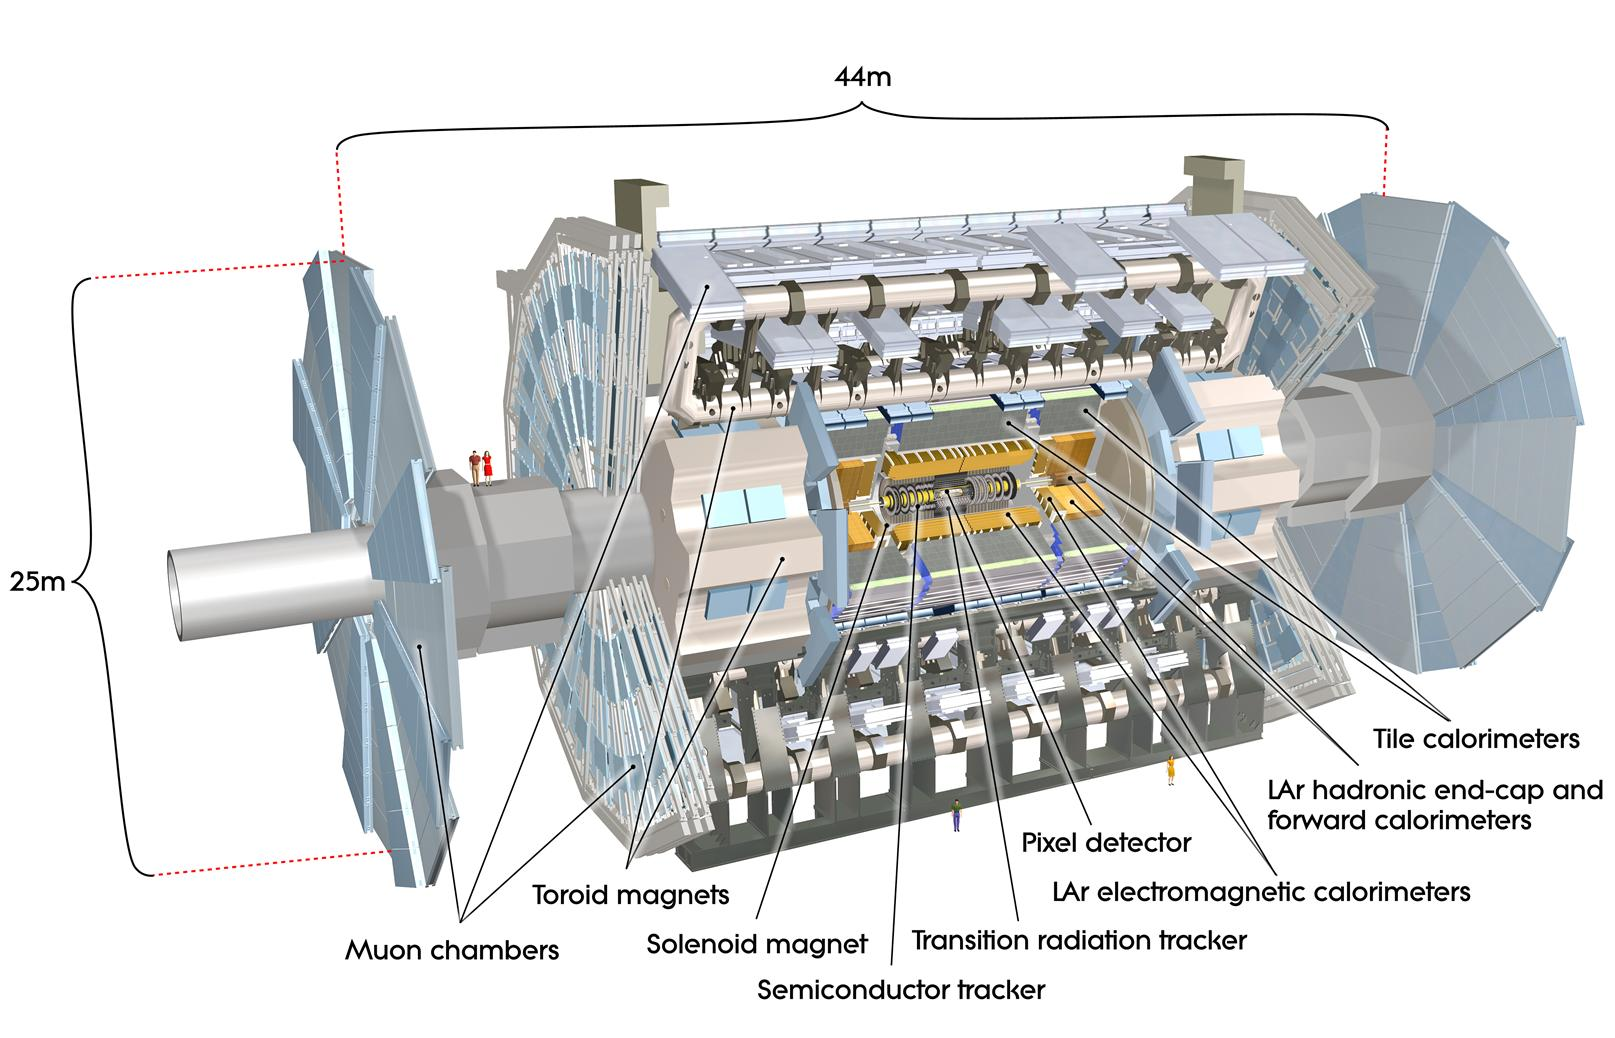
\includegraphics[scale=0.5]{0803012_01-A4-at-144-dpi.jpg}
\caption{Overview of the ATLAS detector~\cite{1748-0221-3-08-S08003}.}
\label{fig:ATLAS_detector}
\end{center}
\end{figure}

The ATLAS detector is designed to record the proton-proton interactions delivered by the LHC.
It can identify particles and measure their tracks and energies with very high precision, therefore, it is sensitive to large areas of particle physics phenomena from the precision measurement of the Standard Model (SM) to beyond the SM.
The detector is constituted by three sub-detector systems and the magnet system.
The innermost part of the detector is called the inner detector which identifies and reconstructs the charged particles as well as the primary and secondary vertices.
Around it, the calorimeter system is built as a cylindrical barrel with caps at each end to measure the particle energies.
The detector is completed by the muon spectrometer which performs identification and measurement of momenta of muons.
The magnetic system produces a field of $B$ = 0.5~T and $B$ = 1~T at barrel and two end-cap, respectively.
The detector has to withstand large collision rates with approximately 1000 particles per collision, therefore, a fast readout and a three-level trigger system are implemented to reduce the event rate from 40~MHz to 200~Hz.
The ATLAS coordinate system and the detail of each sub-detector systems are described in the following sections.

\subsection{The ATLAS coordinate system}

ATLAS uses a right-handed coordinate system with its origin at the nominal proton-proton interaction point (IP) in the centre of the detector and the $z$-axis along the beam pipe.
Along the $z$-axis the detector is divided into side-A (positive $z$) and side-C (negative $z$).
The positive $x$-axis is defined by the direction pointing from the IP to the centre of the LHC ring, and the positive $y$-axis points upward.%Cylindrical coordinates $(r, \phi)$ are used in the transverse plane.
The azimuthal angle $\phi$ is measured around the beam pipe  and the polar angle $\theta$ is the angle from the $z$-axis.
The transverse momentum $p_{\mathrm{T}}$, the transverse energy $E_{\mathrm{T}}$ and the missing transverse
energy $E_{\mathrm{T}}^{\mathrm{miss}}$ are defined in the transverse plane\footnote{$x-y$ plane}, here exemplary for $p_{\mathrm{T}}$:
%
\begin{equation}
p_{\mathrm{T}}= \sqrt{p_{x}^{2} + p_{y}^{2}}
\end{equation}
%
An important quantity in hadron collider physics is the \textbf{rapidity}, $y$, because of the invariance $y$ under Lorentz boosts in the longitudinal direction.
The rapidity is defined as
%
\begin{equation}
y = \frac{1}{2} \ln\Big[\frac{E + p_{z}}{E - p_{z}}\Big]
\end{equation}
%
where $E$ denotes the particle energy and $p_{z}$  is the component of the momentum along the beam direction.
Since mainly leptons can be considered massless in respect to the nominal centre-of-mass energy, the pseudorapidity, $\eta$, is used in stead of using the $y$.
For a massless particle, the \textbf{pseudorapidity}, $\eta$, depends on the polar angle $\theta$ through:
%
\begin{equation}
\eta = - \ln \tan \frac{\theta}{2}
\end{equation}
%
For a particle with the energy $E$ much larger than its mass, the approximation $E \approx |\vec{p}|$ is valid.
The distance, $\Delta R$, between two objects in the $\eta-\phi$ plan is given by
%
\begin{equation}
\Delta R = \sqrt{\Delta \eta^{2} + \Delta \phi^{2}}
\end{equation}
%
where $\Delta \eta$ and $\Delta \phi$ are the difference in pseudorapidity and azimuthal angle, respectively.

\subsection{The Inner Detector and Tracking System}
\label{subsec:inner_detector}

The Inner Detector (ID) consists of three sub-detectors: the Pixel detector, the silicon microstrip trackers  (SCT), and the Transition Radiation Tracker (TRT).
The main purpose of the ID is to provide high precision measurements of the tracks of particles and to reconstruct the primary and secondary vertices.
Each sub-detectors are composed of several layers of material which interacts with the charged particles when the charged particles penetrate the layers.
A  2~T magnetic field generated by the central solenoid parallel to the beam axis is applied to bend the charged particles using the Lorentz force.
By using the radius $r$ of the curvature of the tracks, the magnetic field strength $B$, and the charge of the particle $q$, we can calculate the magnitude of the transverse momentum \pt:
\begin{equation}
\pt = |q|Br
\end{equation}
The layout of the ID is illustrated in Figure~\ref{fig:Inner_detector} and the detail of sub-detectors are described in the following paragraphs.

\begin{figure}[htbp]
\begin{center}
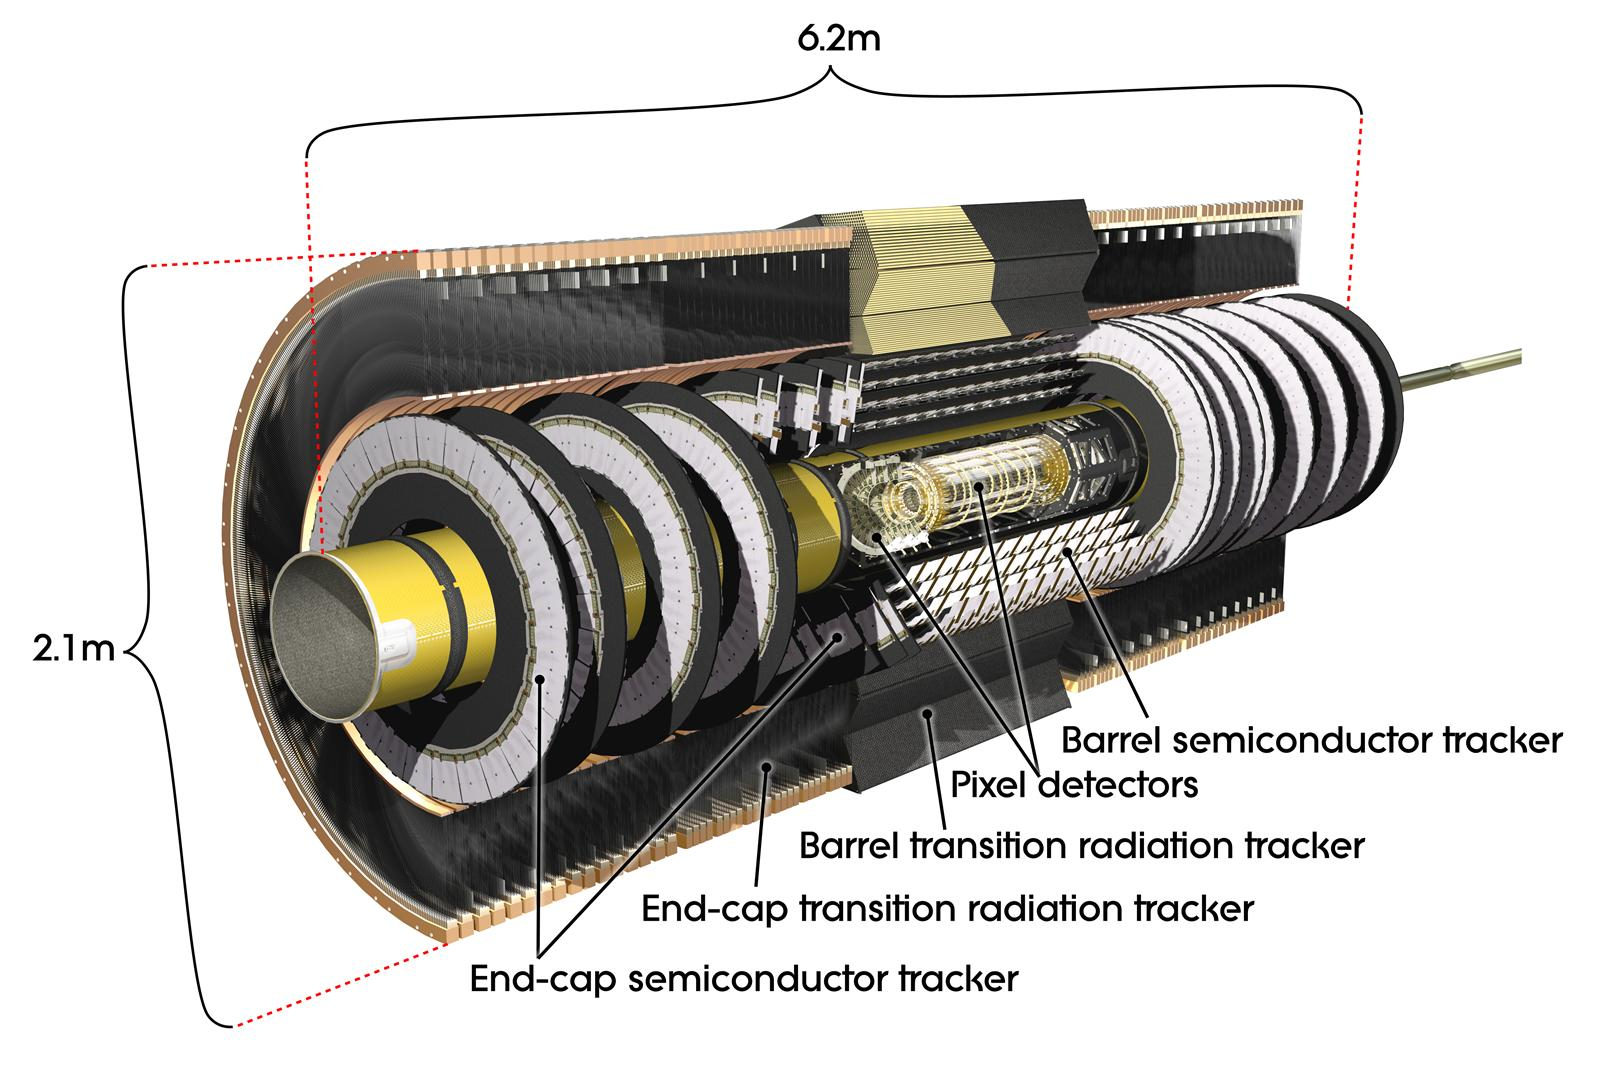
\includegraphics[scale=0.5]{0803014_01-A4-at-144-dpi.jpg}
\caption{Cut-away view of the ATLAS inner detector~\cite{1748-0221-3-08-S08003}.}
\label{fig:Inner_detector}
\end{center}
\end{figure}

%\subsubsection{Pixel Detector}
\noindent \textbf{Pixel Detector}

The innermost part of the entire ATLAS detector components is the Pixel detector which is composed of three barrel layers and three end-cap disks on each side.
The three cylindrical barrel layers around the beam axis have radial positions of 50.5~mm, 88.5~mm, and 122.5~mm respectively and they are made of 22, 38, and 52 identical staves respectively.
Each stave is inclined with azimuthal angle of 20 degrees and is composed of 13 pixel modules with 46,080 readout channel per module.
The size of each pixel is $50 \times 400~\mu m^{2}$ in $R-\phi \times z$.
In the forward region, three disks on each side equip the modules identical to the barrel modules, except the connecting cables. 
The total 1,744 modules in the pixel detector lead to nearly 80 million channel readout and provide the intrinsic accuracies of $10~\mu m$ in $R-\phi$ plane and $115~\mu m$ in $z$ direction covering the region $|\eta| < 2.5$. 

%\subsubsection{Semi Conductor Tracker}
\noindent \textbf{Semi Conductor Tracker}

On the top of the pixel detector is the Semi Conductor Tracker (SCT) which is a silicon strip detector.
There are about 6.3 million readout channels which are arranged in 4088 microstrips.
The intrinsic accuracies per sensor is $17~\mu m$ in $R-\phi$ and $580~\mu m$ in $z$ direction for the barrel and in $R$ for the  disks, respectively.
Similar to the pixel detector, the SCT covers the region $|\eta| < 2.5$ and consists of 8 strip layers in barrel and a total of 9 discs in the end-cap region on each side.
No track reconstruction is possible beyond the covered pseudorapidity range.
Therefore, the electrons cannot be distinguished from photons above $|\eta| > 2.5$ region.

%\subsubsection{Transition Radiation Tracker}
\noindent \textbf{Transition Radiation Tracker}

The outermost component of the ID is the Transition Radiation Tracker (TRT) which consists of 4~mm diameter straw tubes filled with the xenon-based gas mixture.
The gas mixture are ionized by charged particles when they penetrates the straws.
The ionized electrons drift to the cathode because a high voltage is applied on the tungsten wire in the center of the straw tube.
Therefore, the TRT allows the enhanced electron identification, momentum measurement, vertex measurement.
In the barrel region, the straws are surrounded by polypropylene fibres and are divided into two halves at $|\eta|=0$.
In the end-caps, the straws are arranged radially and surrounded by foils as a transition radiation element.
They are read out at two sides and at the center of the TRT with the total number of the readout channels of TRT are approximately 350,000.
The TRT only provides information in the $R-\phi$ plane with an intrinsic accuracy of 130~$\mu$m per straw and covers a range up to $|\eta| < 2.0$. 

%\subsubsection{Solenoid Magnet}
\noindent \textbf{Solenoid Magnet}

A superconducting solenoid magnet encloses the ID and produces a 2~T magnetic field to bend the trajectories of the charged particles.
A cooling system is used and shared with the electromagnetic calorimeter~\ref{subsec:calorimeter} to reduced the deterioration of the energy measurement.

\subsection{The Calorimeters}
\label{subsec:calorimeter}

The calorimeters are used to measure the energy of particles, such as electrons, photons, and jets.
Besides muons, all electromagnetically or haronically interacting particles are stopped in the calorimeters by absorbing their energy.
Not only charged particles but also neutral particles such as photons and neutral hadrons can be detected in the calorimeter.
By requiring highly hermiticity of the calorimeter, the missing energy can be reconstructed precisely as negative vectorial sum of all energy deposits.
The ATLAS Calorimeters system are placed between the Inner Detector~\ref{subsec:inner_detector} and the Muon Spectrometer~\ref{subsec:the_muon_spectrometer}.
The ATLAS calorimeters system consist of an inner Electromagnetic and outer Hadronic Calorimeter together with the Forward Calorimeter.
The Electromagnetic Calorimeter is dedicated for measuring electrons and photons, and the Hadronic Calorimeter focusing on hadronically interacting particles.
The calorimeters cover a range $|\eta| < 4.9$.
An layout view of the ATLAS Calorimeters system is shown in Figure~\ref{fig:calorimeter}

%\subsubsection{Electromagnetic Calorimeter}
\noindent \textbf{Electromagnetic Calorimeter}

The Electromagnetic Calorimeters (ECAL) measure the energy of electrons and photons as they interact with matter.
The ECAL consists of layers of high-density material, lead, as absorbers and interleaved with layers of liquid argon (LAr) as active medium.





%\subsubsection{Hadronic Calorimeter}
\noindent \textbf{Hadronic Calorimeter}


Hadrons, which are signi cantly heavier and mainly interact via the strong force, propagate further causing more wide-spread hadronic showers mainly in the denser Hadronic Calorimeter.

%\subsubsection{Forward Calorimeter}
\noindent \textbf{Forward Calorimeter}


\begin{figure}[htbp]
\begin{center}
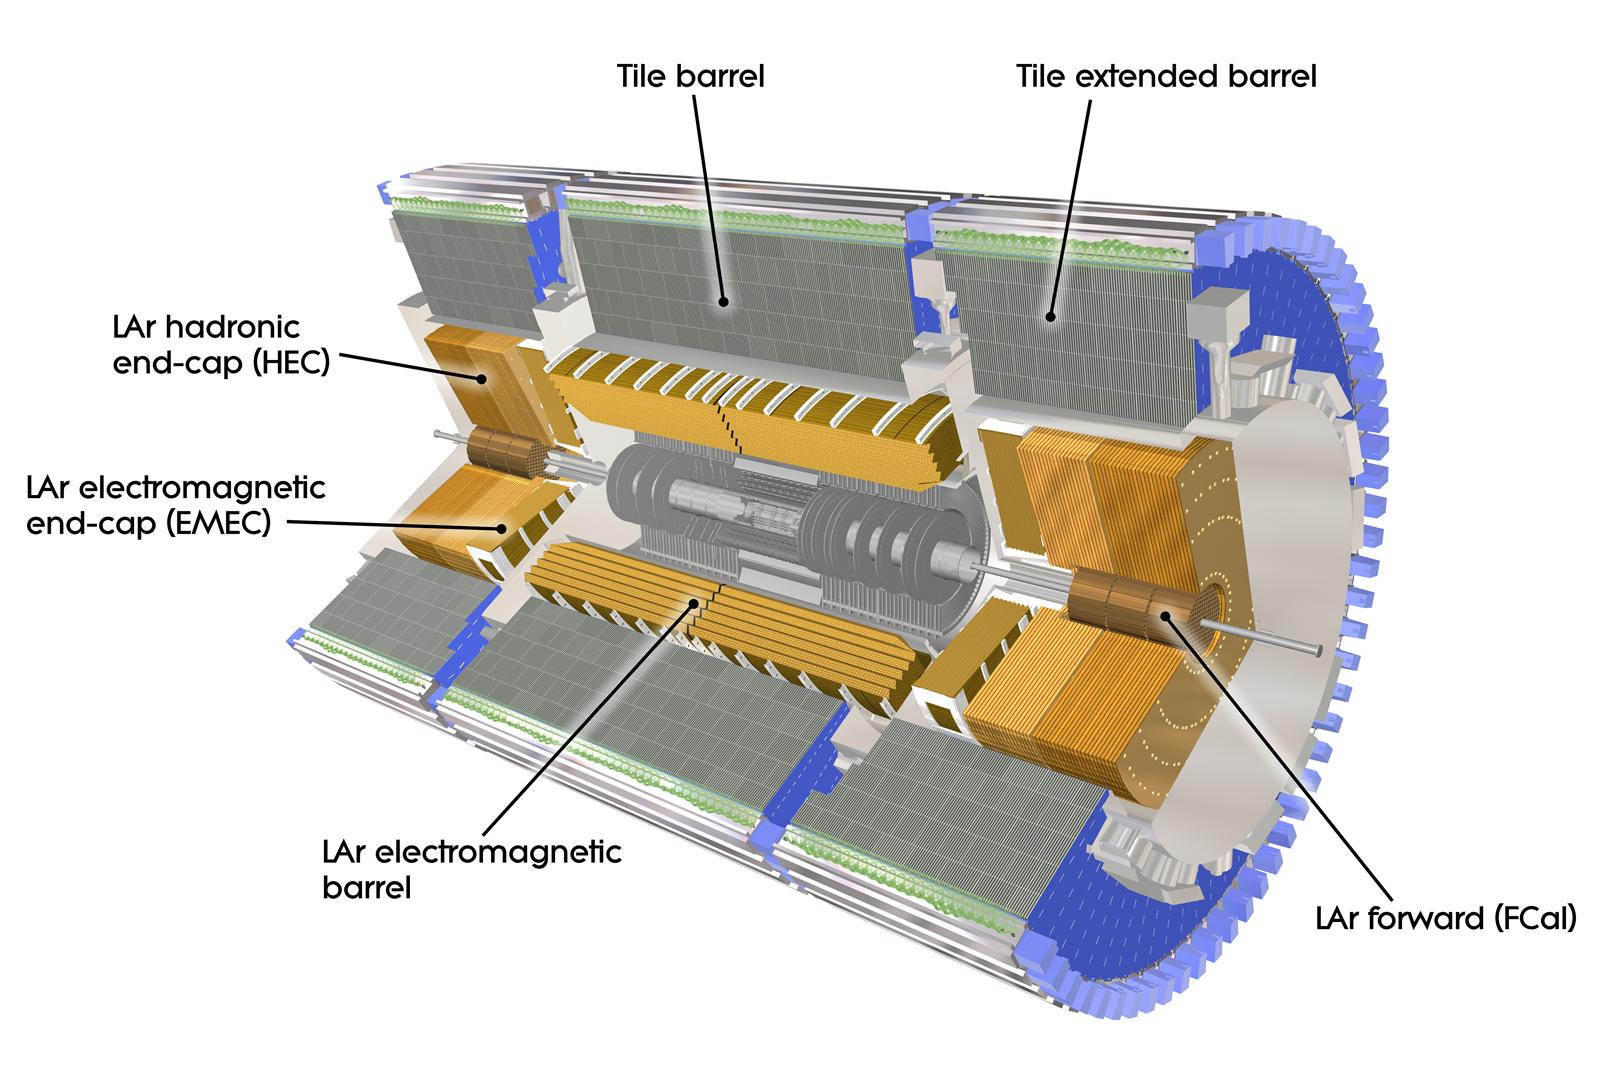
\includegraphics[scale=0.5]{0803015_01-A4-at-144-dpi.jpg}
\caption{Cut-away view of the calorimeter system~\cite{1748-0221-3-08-S08003}.}
\label{fig:calorimeter}
\end{center}
\end{figure}

\begin{table}[htbp]
\begin{center}
\begin{tabular}{cc}
\hline
\hline
Calorimeter & Required resolution\\
\hline
ElectromagneticCalorimeter & $\sigma_{E}/E = 10\% / \sqrt{E\mathrm{ (GeV)}} \oplus 0.7\%$\\
Hadronic Calorimeter & $\sigma_{E}/E = 50\% / \sqrt{E~\mathrm{(GeV)}} \oplus 3\%$\\
Forward Calorimeter & $\sigma_{E}/E = 100\% / \sqrt{E~\mathrm{(GeV)}} \oplus 10\%$\\
\hline
\hline
\end{tabular}
\end{center}
\caption{Resolution requirements for the different calorimeters of the ATLAS detector~\cite{1748-0221-3-08-S08003}.}
\label{tab:}
\end{table}%







\subsection{The Muon Spectrometer} \label{subsec:the_muon_spectrometer}

The outermost part of the ATLAS detector is the Muon Spectrometer~\cite{1748-0221-3-08-S08003}~\cite{Palestini:681459}~\cite{0910.2767}.
Muons have the same properties as electrons but 200 times heavier than the electrons and muons don't interact predominately by Bremsstrahlung but have minimal ionizing at LHC energy in the inner layers of the detector.
Only the muons with an energy less than 5~{\GeV} are stopped before the Muon Spectrometer.
Therefore, muons are the only measurable particles that can penetrate the Inner Detector and the Calorimeters.
In order to determine the muon momentum with high precision, a detector that concentrates on the measurement of muons is necessary.

The Muon Spectrometer is designed to measure the transverse momentum ($p_{\mathrm{T}}$) of muons with $p_{\mathrm{T}} > 3$~{\GeV} with a resolution of 3\% for $p_{\mathrm{T}} < 250$~{\GeV} and increasing to 10\% at 1~{\TeV}.
It consists of large toroid magnets system and three layers of high precision tracking chambers which allow a precise measurement of the muon momentum over nearly the full solid angle.
The barrel toroid magnet system is composed of eight superconducting coils which are installed radial symmetrically around the beam pipe.
It covers the range $|\eta| < 1.4$ and bends the trajectories of muons with the bending power 1.5 to 5.5 Tm.
The magnetic field produced by the barrel toroid magnets provides an approximately 1~T field at the center of each coils, but is rather non-uniform, especially in the barrel-endcap transition region.
In the endcap toroid magnets system, the magnetic field is provided by eight superconducting coils, closed in an insulation vessel extending to about 10 m in diameter, located between the first and the second station of tracking chambers.
The endcap toroid magnets cover $1.6 < |\eta| < 2.4$ and provide a a magnetic field in the range of 1 to 2 T with bending power 1 to 7.5 Tm.

The Monitored Drift Tubes (MDTs) consists of cylindrical drift tubes, filled with a gas mixture of argon and carbon dioxide.
A tungsten-rhenium alloyed aluminium wire in the centre of each tube collects the electrons freed by ionization of the gas volume by traversing muons.
The MDTs covers a full range of $|\eta| < 2.7$, while the inner layer only covers $|\eta| < 2.0$.
The Cathode Strip Chambers (CSCs) provides a coverage range $2.0 < |\eta| < 2.7$, where MDTs would have occupancy problems.
Both MDTs and CSCs are used for precision tracking in the spectrometer bending plane and end-cap inner layer, respectively.
The Resistive Plate Chambers (RPCs) and Thin Gap Chambers (TGCs) are used for triggering in barrel and end-cap, they have sufficient intrinsic time resolution of 1.5 ns and 4 ns, respectively.
A sketch of the Muon Spectrometer and its four components are depicted in Figure~\ref{fig:muon_spectrometer} and Table~\ref{tab:muon_spectrometer_components} gives a summary of the Muon Spectrometer components

\begin{figure}[htbp]
\begin{center}
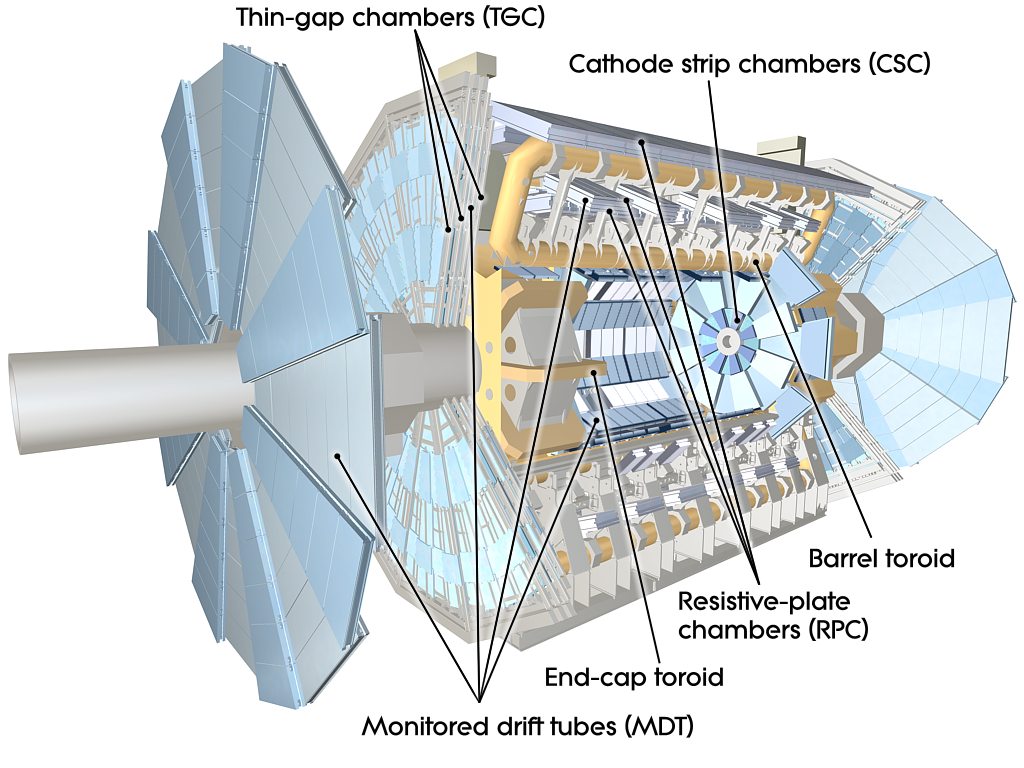
\includegraphics[scale=0.4]{MuonSystem_d3.png}
\caption{Sketch of the muon system of the ATLAS detector~\cite{1748-0221-3-08-S08003}.}
\label{fig:muon_spectrometer}
\end{center}
\end{figure}

\begin{table}[htbp]
\begin{center}
\begin{tabular}{ccccc}
\hline
\hline
Type & Purpose & Location & $\eta$ coverage & Channel\\
\hline
MDT & Tracking & barrel + end-cap & $0.0 < \eta < 2.7$ & 354k\\
CSC & Tracking & end-cap layer 1 & $2.0 < \eta < 2.7$ & 30.7k\\
RPC & Trigger & barrel & $0.0 < \eta < 1.0$ & 373k\\
TGC & Trigger & end-cap & $1.0 < \eta < 2.4$ & 318k\\
\hline
\hline
\end{tabular}
\end{center}
\caption{A summary of the Muon Spectrometer components.}
\label{tab:muon_spectrometer_components}
\end{table}%

\subsection{The Trigger System and Data Acquisition}

\subsection{}



\chapter{The Electron Isolation Efficiency and Scale Factors}
\label{chapter:electron_isolation}
\graphicspath{{figures/electron_isolation}}
\input{chapter_electron_isolation}


\chapter{The Real Lepton Efficiencies}
\label{chapter:real_lepton_efficiencies}
\graphicspath{{figures/real_lepton_efficiencies}}
\input{chapter_real_lepton_efficiencies}

\chapter{Results}
\label{chapter:results}
\graphicspath{{figures/results/}}
A search for the electroweak production of supersymmetric states with low \pt visible decay products is presented.
Events with significant \met and same flavor opposite charged lepton pairs are selected.
The minimum \pt of the lepton is 4.5~{\GeV} for the electrons and 4~{\GeV} for the muons.
The dilepton invariant mass and stranverse mass are the main discriminating variables used to construct signal regions.
This analysis is performed using LHC proton-proton collision data at $\sqrt{s} = 13$~{\TeV} collected by the ATLAS detector corresponding to an integrated luminosity of 36.1~\ifb.
Since no excess over the Standard Model expectation is observed, the results are interpreted using $R$-parity-conserving supersymmetry, where the produced states have small mass splitting with the lightest neutralino $\widetilde{\chi}^{0}_{1}$.
For the NUHM2 scenario, 95\% CL cross-section upper limits ranging between 11.5 and 3.8 pb for $m_{1/2}$ values of 350 to 800~{\GeV} are provided.


%\FloatBarrier


\chapter{Conclusion}
\label{chapter:conclusion}
\graphicspath{{figures/conclusion/}}
A search for the electroweak production of supersymmetric states with low \pt visible decay products is presented.
Events with significant \met and same flavor opposite charged lepton pairs are selected.
The minimum \pt of the lepton is 4.5~{\GeV} for the electrons and 4~{\GeV} for the muons.
The dilepton invariant mass and stranverse mass are the main discriminating variables used to construct signal regions.
This analysis is performed using LHC proton-proton collision data at $\sqrt{s} = 13$~{\TeV} collected by the ATLAS detector corresponding to an integrated luminosity of 36.1~\ifb.
Since no excess over the Standard Model expectation is observed, the results are interpreted using $R$-parity-conserving supersymmetry, where the produced states have small mass splitting with the lightest neutralino $\widetilde{\chi}^{0}_{1}$.
For the NUHM2 scenario, 95\% CL cross-section upper limits ranging between 11.5 and 3.8 pb for $m_{1/2}$ values of 350 to 800~{\GeV} are provided.


%------------------------------------------------------------------------------- 
\clearpage

%\appendix
%\part*{Appendix}
%\addcontentsline{toc}{part}{Appendix}

%\section{Simulated samples, cross-sections and equivalent luminosities}
%\label{app:samples}
%The Monte Carlo (MC) samples are used to model the SUSY signals and to estimate the SM background.
The MC samples are processed using a ATLAS detector full simulation (FullSim) or a fast simulation (AFII\footnote{AFII stands for ATLAS Fast II.}) based on {\GEANT}4~\cite{Agostinelli:2002hh} simulation package.
The FullSim simulates the detailed properties of the ATLAS detector while the AFII uses a parameterized calorimeter response and simulates ID and MS~\cite{ATLAS:1300517} based on {\GEANT}4.
The simulated MC events are reweighted to the observed pile-up conditions in the data.

%%%
%%%
%%%

\section{Samples used for strong interaction}
\label{sec:app_samples_strong}

Table~\ref{tab:app_sample_strong} shows the event generator, parton shower, cross-section normalization, PDF set~\cite{Martin:2009iq}, and the set of tunned parameters for modelling for all samples.
Except those produced by the {\SHERPA}, the \textsc{EvtGEN}\xspace v1.2.0 package~\cite{Lange:2001uf} is used to model the properties of bottom and charm hadron decays for all MC samples.

\begin{table}[htp]
%\begin{center}
\resizebox{\textwidth}{!}{% <------ Don't forget this %
\begin{tabular}{ccccccc}
\hline
\hline
Signal/Background                                      & Physics process                   & Event generator                  & Parton shower     & Cross-section normalization & PDF set    & Set of tunned parameters\\
\hline
\hline
\multirow{3}{*}{Signal}                                & RPC                               & MG5\_{\scriptsize A}MC@NLO 2.2.3 & {\PYTHIA} 8.186   & NLO+NLL                     & NNPDF2.3LO & A14\\
                                                       & RPV (except Figure~\ref{})        & MG5\_{\scriptsize A}MC@NLO 2.2.3 & {\PYTHIA} 8.210   & or                          & NNPDF2.3LO & A14\\
                                                       & RPV (Figure~\ref{})               & {\HERWIGpp} 2.7.1                & {\HERWIGpp} 2.7.1 & NLO-Prospino2               & CTEQ6L1    & UEEE5\\
\hline
\multirow{3}{*}{\shortstack{$t\bar{t}+X$\\background}} & $t\bar{t}W, t\bar{t}Z/\gamma^{*}$ & MG5\_{\scriptsize A}MC@NLO 2.2.2 & {\PYTHIA} 8.186   & NLO                         & NNPDF2.3LO & A14\\
                                                       & $t\bar{t}H$                       & MG5\_{\scriptsize A}MC@NLO 2.3.2 & {\PYTHIA} 8.186   & NLO                         & NNPDF2.3LO & A14\\
                                                       & 4$t$                              & MG5\_{\scriptsize A}MC@NLO 2.2.2 & {\PYTHIA} 8.186   & NLO                         & NNPDF2.3LO & A14\\
\hline
\multirow{2}{*}{\shortstack{Dibosno\\background}}      & $ZZ, WZ$                          & {\SHERPA} 2.2.1                  & {\SHERPA} 2.2.1   & NLO                         & NNPDF2.3LO & {\SHERPA} default\\
                                                       & Other (inc. $W^{\pm}W^{\pm}$)     & {\SHERPA} 2.1.1                  & {\SHERPA} 2.1.1   & NLO                         & CT10       & {\SHERPA} default\\
\hline
\multirow{4}{*}{\shortstack{Rare\\background}}         & $t\bar{t}WW, t\bar{t}WZ$          & MG5\_{\scriptsize A}MC@NLO 2.2.2 & {\PYTHIA} 8.186   & NLO                         & NNPDF2.3LO & A14\\
                                                       & $tZ, tWZ, tt\bar{t}$              & MG5\_{\scriptsize A}MC@NLO 2.2.2 & {\PYTHIA} 8.186   & LO                          & NNPDF2.3LO & A14\\
                                                       & $WH, ZH$                          & MG5\_{\scriptsize A}MC@NLO 2.2.2 & {\PYTHIA} 8.186   & NLO                         & NNPDF2.3LO & A14\\
                                                       & Triboson                          & {\SHERPA} 2.1.1                  & {\SHERPA} 2.1.1   & NLO                         & CT10       & {\SHERPA} default\\
\hline
\hline
\end{tabular}
%\end{center}
}
\caption{The simulated signal and background MC samples.
The event generator, parton shower, cross-section normalization, PDF set, and the set of tunned parameters for each samples are shown.
The $t\bar{t}WW, t\bar{t}WZ, tZ, tWZ, tt\bar{t}, WH, ZH$ and triboson background samples are labeled in the "rare" because they contribute a very small amount to the signal region.}
\label{tab:app_sample_strong}
\end{table}%


%%%
%%%
%%%

\section{Samples used for weak interaction}
\label{sec:app_samples}

%%%
%%%
%%%
%\clearpage
%-------------------------------------------------------------------------------

\clearpage

%\printbibliography
\clearpage










\bibliographystyle{unsrt}
%% You need a file named `outhesis_references.bib' to use BibTex here
%\bibliography{outhesis_references}
\bibliography{bib_atlas_experiment}



% \appendix{A}
% \input{appendices/appendixA}
%\begin{appendices}
%\input{chapter_hardware}
%\input{chapter_auxiliaryPlots8TeV}
%\input{chapter_JSSuncSmoothing}
%\end{appendices}


% \backmatter


\end{document}

